\section{Ceрвер jabber.org.by/jabber.linux.by}
\begin{frame}{О сервере}
  Первый, и единственный публичный сервер в РБ.

  Особенности:
  \begin{itemize}
      \item открытая регистрация
      \item community-driven
      \item широкий набор транспортов\footnote{ICQ, MSN, AIM, Yahoo, Twitter, MRIM и несколько транспортов в XMPP под разными именами}
      \item физически расположен в Беларуси \footnote{провайдер BASNET} 
  \end{itemize}

  Опыт поддержки и эксплуатации указанного сервера в течении 9 лет и положен в основу доклада.
\end{frame}

\begin{frame}{Hardware und Software}

  \begin{block}{Hardware} 
    \begin{itemize}
      \item Контейнер в OpenVZ
      \item RAM 2GB\footnote{до 4GB если другие контейнеры не требуют}  
      \item 40 GB HDD
      \item Intel(R) Xeon(R) CPU E5506  @ 2.13GHz  
    \end{itemize} 
  \end{block}
 
  \pause
  
  \begin{block}{Software}
    \begin{itemize}
      \item Debian GNU/Linux 7.x (stable)
      \item jabberd: Prosody 0.9
      \item транспорты Spectrum2
    \end{itemize}
  \end{block}
\end{frame}

\subsection{Вехи развития jabber.org.by}

\begin{frame}{Начало}
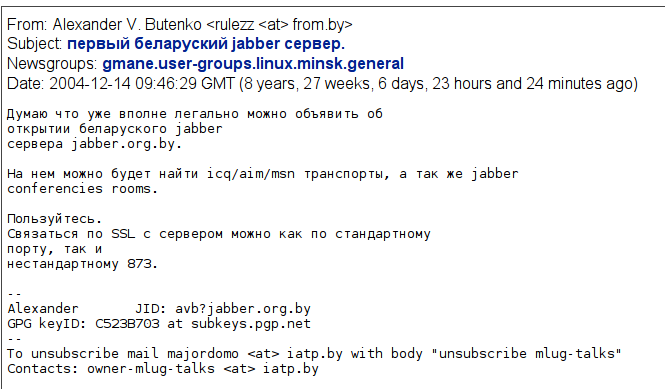
\includegraphics[width=10cm]{beginning}
\end{frame}

\begin{frame}{События}

  \begin{itemize}
    \item 14 декабря 2004 года. Запуск.
    \item конец 2005. Пользователи (cympak, booxter, trenka) по своей инициативе собирают деньги и апгрейдят сервер.
    \item 14.12.2006 Внутренний hackaton по исправлению утечек памяти в PyICQt.  
    \item 09.03.2007. Эмиграция MrDeath в Доминиканскую Республику
    \item март 2008. Остановка сервиса и далее переезд на FreeBSD
    \item август 2009. тестированиe под нагрузкой и исправлении утечки памяти в PyICQt 0.8.1.5
    \item февраль 2011. Переезд на Debian 6.x/OpenVZ. Переход на сервисы Spectrum.
    \item сентябрь 2012-май 2013. Эпическая Борьба с сирийскими ботами.
    \item июнь 2013. Потеря пользовательских паролей (неудачный апдейт)
    \item 14 июня 2013. Переход на Prosody.
  \end{itemize}

\end{frame}

\begin{frame}{MrDeath: Привет из Доминиканы - 1}
  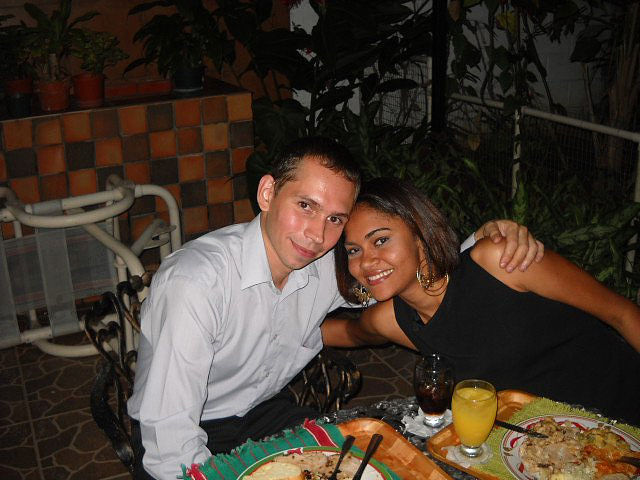
\includegraphics[width=10cm]{avb_with_Karla}
\end{frame}

\begin{frame}{MrDeath: Привет из Доминиканы - 2}
  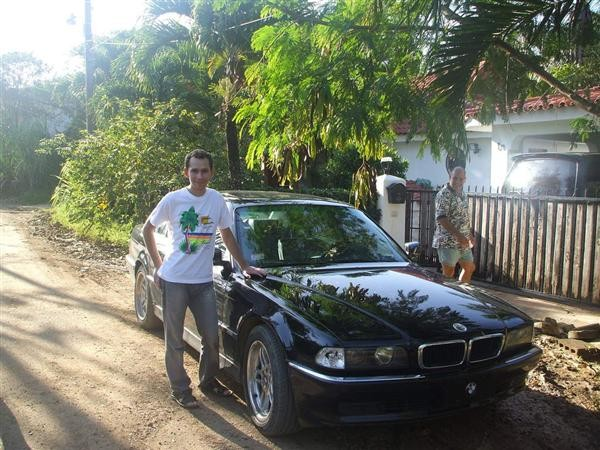
\includegraphics[width=10cm]{avb_with_black_boomer}
\end{frame}

\begin{frame}{Текущий статус сервера}
   \begin{itemize}
      \item учётки @jabber.org.by и @jabber.linux.by
      \item ~ 50-70 активных пользователей
      \item S2S - 130-150 одновременно
      \item транспорты - до 400 юзеров одновременно
    \end{itemize}
\end{frame}


